\section{Validation of the Estimator and of the Intervals}
\label{sec:validation}
\label{app:ext_valid}
\emph{In short: toy-MC experiments generated from the fitted model show that the maximum-likelihood estimate of $A$ is unbiased and attains the minimum variance bound, that the Wilks interval has the nominal coverage, and that the test of $A=0$ has the expected size and a power that is known as a function of the injected asymmetry.}

The asymptotic properties of the maximum-likelihood estimator and of the profile-likelihood ratio were verified on toy-MC experiments generated from the fitted model (Sec.~\ref{sec:validation_toys}), which allow the true value of $A$ to be chosen.

\subsection{Generation of the Toy-MC Experiments}
\label{sec:validation_toys}
\emph{In short: toy experiments are generated from the fitted model (Poisson yields, masses by the transformation method) and fitted with the nominal procedure: $1000$ at the fitted value and $300$ at each of four other values of $A$.}
The Frequentist results of Sec.~\ref{sec:frequentist} rest on asymptotic properties of the maximum-likelihood estimator and of the profile-likelihood ratio, and Sec.~\ref{sec:freq_coverage} verified the coverage by resampling the data. Here the same questions are asked of toy-MC experiments generated from the fitted model, as was done for the Bayesian interval in Sec.~\ref{sec:bayes_toymc}, which allows the true value of $A$ to be chosen. The fitted model of Sec.~\ref{sec:model} defines the toy-MC datasets: for each charge the yields of signal and background are Poisson-fluctuated, the signal masses are drawn from the truncated Gaussian and the background masses from the two truncated exponentials by the transformation method. Each dataset is fitted with the nominal Frequentist procedure; the likelihood ratio $t(A_{\mathrm{true}})=-2\ln[L(A_{\mathrm{true}})/L(\hat A)]$ and the statistic of the test of $A=0$, $q(0)$, are computed with the other eleven parameters profiled. One thousand toy-MC experiments were generated at the fitted value, $A_{\mathrm{true}}=-0.0441$, and $300$ at each of $A_{\mathrm{true}}=-0.1$, $-0.02$, $0$ and $+0.05$; between $1\%$ and $3\%$ of the fits are not flagged as valid by \texttt{MIGRAD} and are excluded.

\subsection{Bias, Efficiency and Coverage}
\label{sec:validation_estimator}
\emph{In short: no bias larger than $0.0008$, an estimator spread equal to the Hesse uncertainty within $6\%$, and coverage of $0.70\pm0.01$ and $0.95\pm0.01$ at the fitted value; the test of $A=0$ has size $0.051\pm0.013$ and power $0.68$ at $A=-0.02$.}
Table~\ref{tab:validation_toys} summarizes the estimator over the five injected values: the bias of $\hat A$ is at most $0.0008$ ($1.6$ standard errors), its spread equals the mean Hesse uncertainty within $6\%$ and the pulls have width $0.94$--$1.05$, so the estimator is unbiased and reaches the minimum variance bound. At the fitted value the coverage of $t(A_{\mathrm{true}})\leq1$ is $0.696\pm0.015$ ($68.3\%$ level) and $0.954\pm0.007$ ($95.4\%$ level); at $A_{\mathrm{true}}=+0.05$ the $68\%$ coverage is $0.614\pm0.028$, $2.5$ standard deviations low, not unexpected among five values.

\begin{table}[h]
\centering
\resizebox{\ifdim\width>\linewidth\linewidth\else\width\fi}{!}{\begin{tabular}{rrcccc}
\toprule
$A_{\mathrm{true}}$ & $n$ & bias & sd$(\hat A)/\langle\sigma_{\mathrm{Hesse}}\rangle$ & cov.\ $68\%$ & cov.\ $95\%$ \\
\midrule
$-0.1$ & $297$ & $-0.0005\pm0.0005$ & $0.94$ & $0.71$ & $0.96$ \\
$-0.0441$ & $985$ & $-0.0001\pm0.0003$ & $0.97$ & $0.70$ & $0.95$ \\
$-0.02$ & $290$ & $-0.0008\pm0.0005$ & $1.02$ & $0.69$ & $0.94$ \\
$0$ & $293$ & $+0.0002\pm0.0005$ & $1.01$ & $0.69$ & $0.95$ \\
$+0.05$ & $293$ & $-0.0004\pm0.0005$ & $1.05$ & $0.61$ & $0.96$ \\
\bottomrule
\end{tabular}}
\caption{Toy-MC experiments at five injected values of the asymmetry: number of valid fits, bias of $\hat A$ with its standard error, spread of the estimates relative to the mean Hesse uncertainty ($0.0085$), and coverage of the intervals $t(A_{\mathrm{true}})\leq1$ and $\leq3.84$.}
\label{tab:validation_toys}
\end{table}

Together, the estimator is unbiased and efficient, the interval has its nominal coverage and the test its nominal size (Sec.~\ref{sec:validation_power}); the $5.2\sigma$ of the data is an extrapolation of the $\chi^2_1$ tail, which the $293$ experiments check only down to the $3\sigma$ level.




\subsection{Asymptotic Behavior of the Estimator}
\label{sec:checks_scaling}
\emph{In short: with the number of candidates the bias tends to zero, the spread scales as $N^{-1/2}$ and the distribution of $\hat A$ becomes Gaussian, as the central limit theorem and the asymptotic properties of the maximum-likelihood estimate predict.}
The $300$ toy-MC datasets for each size of the low-statistics study (Sec.~\ref{sec:bayes_lowstat}) show the approach to the asymptotic limit (Table~\ref{tab:checks_scaling}): the bias decreases from $-0.0085$ at $N=50$ to $+0.0009$ at $N=2000$, the product of the spread and $\sqrt N$ is constant, and the distribution of $\hat A$ is compatible with a Gaussian from $N=150$ (Shapiro-Wilk $p>0.3$), with a mild excess kurtosis at $N=50$ ($p=0.03$). Linear propagation of the Poisson uncertainty of the signal yield, $\sigma(A)=\sqrt{(1-A^2)/N_s}$ with $N_s=0.86\,N$, gives $0.153$ at $N=50$ and $0.024$ at $N=2000$, against spreads of $0.161$ and $0.023$: it is correct at the few-per-cent level, because the fit also has to determine the background, and the first-order expansion is not the limiting approximation. At the full sample the spread of the estimator equals the Hesse uncertainty (Sec.~\ref{sec:validation_estimator}).

\begin{table}[h]
\centering
\resizebox{\ifdim\width>\linewidth\linewidth\else\width\fi}{!}{\begin{tabular}{rcccccc}
\toprule
$N$ & bias & sd$(\hat A)$ & sd$\cdot\sqrt N$ & skewness & ex.\ kurtosis & Shapiro $p$ \\
\midrule
$50$ & $-0.0085$ & $0.1611$ & $1.14$ & $-0.15$ & $+0.64$ & $0.03$ \\
$150$ & $-0.0051$ & $0.0920$ & $1.13$ & $+0.16$ & $+0.31$ & $0.59$ \\
$500$ & $-0.0022$ & $0.0501$ & $1.12$ & $-0.08$ & $+0.38$ & $0.52$ \\
$2000$ & $+0.0009$ & $0.0225$ & $1.01$ & $-0.20$ & $-0.20$ & $0.32$ \\
\bottomrule
\end{tabular}}
\caption{Distribution of the maximum-likelihood estimate of $A$ in $300$ toy-MC datasets of $N$ candidates (six-parameter model of Sec.~\ref{sec:bayes_minimal}).}
\label{tab:checks_scaling}
\end{table}

\subsection{Size and Power of the Test of $A=0$}
\label{sec:validation_power}
\emph{In short: the test has the nominal size, the statistic $q(0)$ follows a $\chi^2$ distribution with one degree of freedom, and an asymmetry of $-0.02$ would be rejected at $3\sigma$ in one toy-MC experiment out of four.}
Under $A_{\mathrm{true}}=0$ the fraction of toy-MC experiments with $q(0)>3.84$ is $0.051\pm0.013$, against the nominal size $\alpha=0.05$, and $2$ of $293$ exceed $q=9$ ($3\sigma$), against the $0.8$ expected; the distribution of $q(0)$ is compatible with $\chi^2_1$ (Kolmogorov-Smirnov $p=0.79$, Fig.~\ref{fig:validation_null}a), and the tail used for the significance ($q=27$) is an extrapolation of it. The power, the probability of rejecting $A=0$ when the asymmetry is $A_{\mathrm{true}}$ (Fig.~\ref{fig:validation_injection}c), is $1.00$ at the fitted value and at $\pm$ the larger injected values, and $0.68$ ($0.27$ at $3\sigma$) at $A_{\mathrm{true}}=-0.02$: with $19{,}731$ candidates an asymmetry of $0.02$ is detected in about two experiments out of three at the $5\%$ size, and an asymmetry below that is not resolved.

\begin{figure*}[!t]
\centering
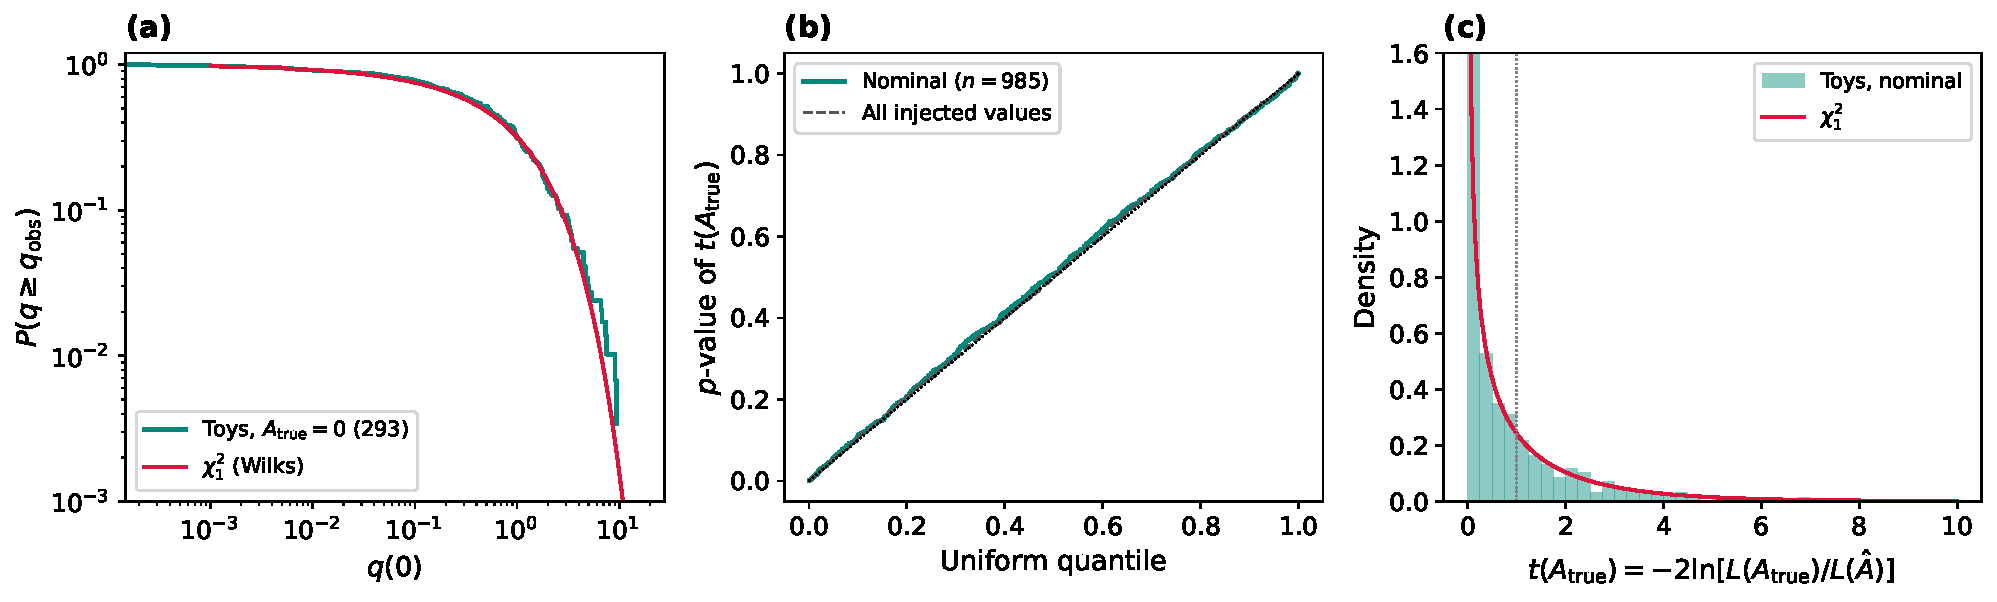
\includegraphics[width=0.95\textwidth]{figures/validation_null_wilks.pdf}
\caption{Toy-MC experiments, validity of Wilks' theorem. (a) Fraction of experiments with $q(0)$ above the observed value, for $A_{\mathrm{true}}=0$, compared with the $\chi^2_1$ distribution. (b) $p$-value of $t(A_{\mathrm{true}})$ against a uniform distribution, at the fitted value and pooled over the injected values. (c) Distribution of $t(A_{\mathrm{true}})$ at the fitted value and $\chi^2_1$.}
\label{fig:validation_null}
\end{figure*}



\begin{figure*}[!t]
\centering
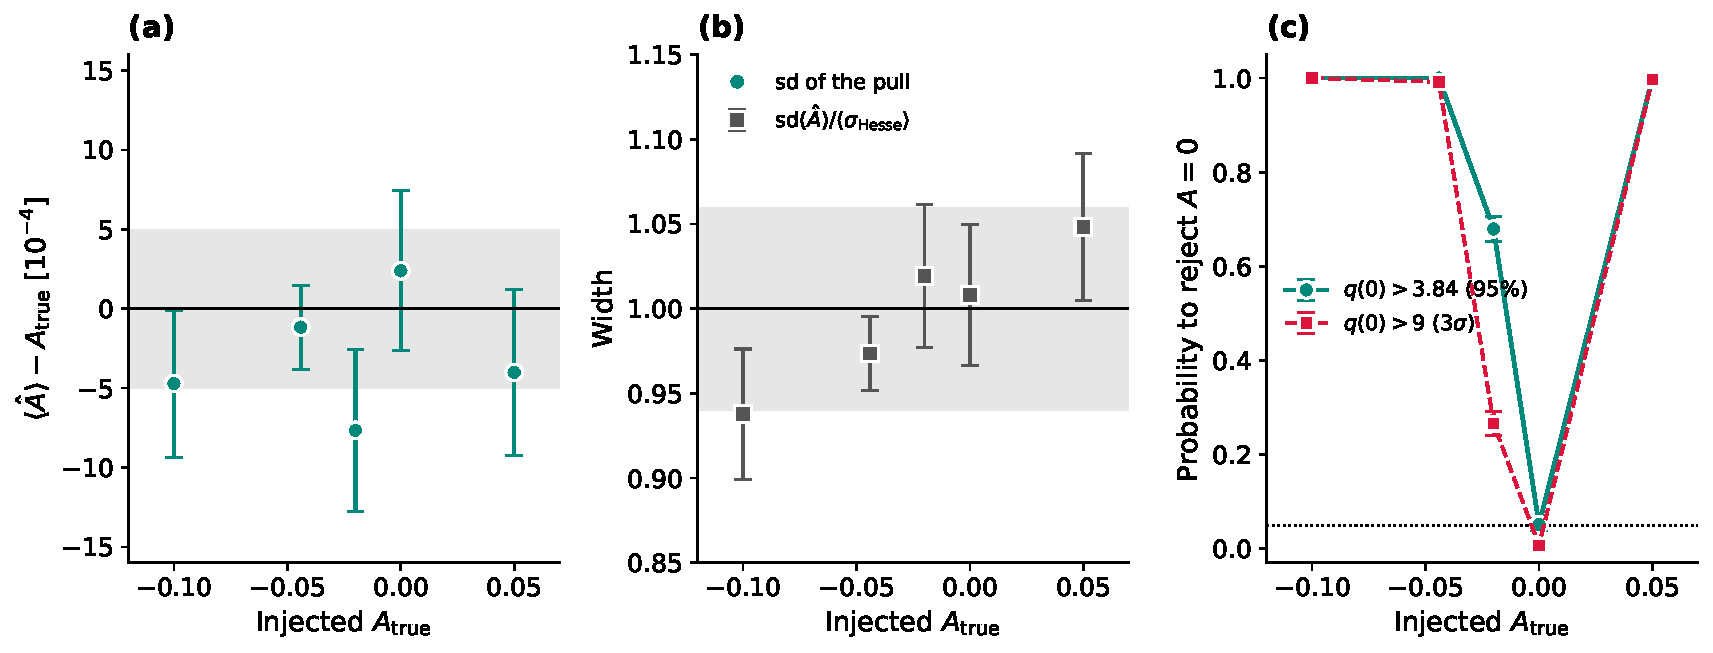
\includegraphics[width=0.95\textwidth]{figures/short_injection_power.pdf}
\caption{Toy-MC experiments at five injected asymmetries. (a) Bias of $\hat A$, with its standard error. (b) Spread of the estimates divided by the mean Hesse uncertainty, and width of the pulls. (c) Probability to reject $A=0$ in the test with $q(0)>3.84$ (size $5\%$) and $q(0)>9$ ($3\sigma$), as a function of the injected value: size at $A_{\mathrm{true}}=0$, power elsewhere.}
\label{fig:validation_injection}
\end{figure*}

\subsection{Goodness of Fit and the Binning}
\label{sec:validation_gof}
\emph{In short: the binned $\chi^2$ of toy-MC experiments follows its asymptotic distribution, so its $p$-values are accurate; the misfit of the data is $5.4$ standard deviations at $10\,\MeV$ bins and $2.0$ at $2.5\,\MeV$, because it lives on the scale of the flanks of the peak.}
The $p$-values of the binned $\chi^2$ rely on the asymptotic distribution with $\mathrm{ndof}$ degrees of freedom, which can fail for bins with few entries. The $\chi^2$ of $1000$ toy-MC experiments from the fitted model has mean $87.6$ and standard deviation $13.3$ for $2\times50$ bins ($88$ degrees of freedom, expected $\sqrt{2\cdot88}=13.3$), and mean $387.6$, standard deviation $27.1$ for $2\times200$ bins ($388$ degrees of freedom): the asymptotic $\chi^2$ distribution describes the toys (Fig.~\ref{fig:validation_gof}). The data give $159.5$ for $2\times50$ bins of $10\,\MeV$, $5.4$ standard deviations above the toys (asymptotic $p=4.8\times10^{-6}$, fewer than $1/1000$ toys above), $253.1/188$ for $5\,\MeV$ bins ($p=1.1\times10^{-3}$) and $441.7/388$ for $2.5\,\MeV$ bins ($2.0$ standard deviations, $p=0.031$, in toys $0.032$). The same fit therefore has $p=0.03$ or $p=5\times10^{-6}$ depending on the binning: the discrepancy between model and data is a feature of $\sim10\,\MeV$ width, the flanks of the peak (Fig.~\ref{fig:bayes_fit}), diluted in narrower bins, and the binned $\chi^2$ is a test whose power depends on the binning, in the same way as the Bayes factor depends on the prior width.

\begin{figure*}[!t]
\centering
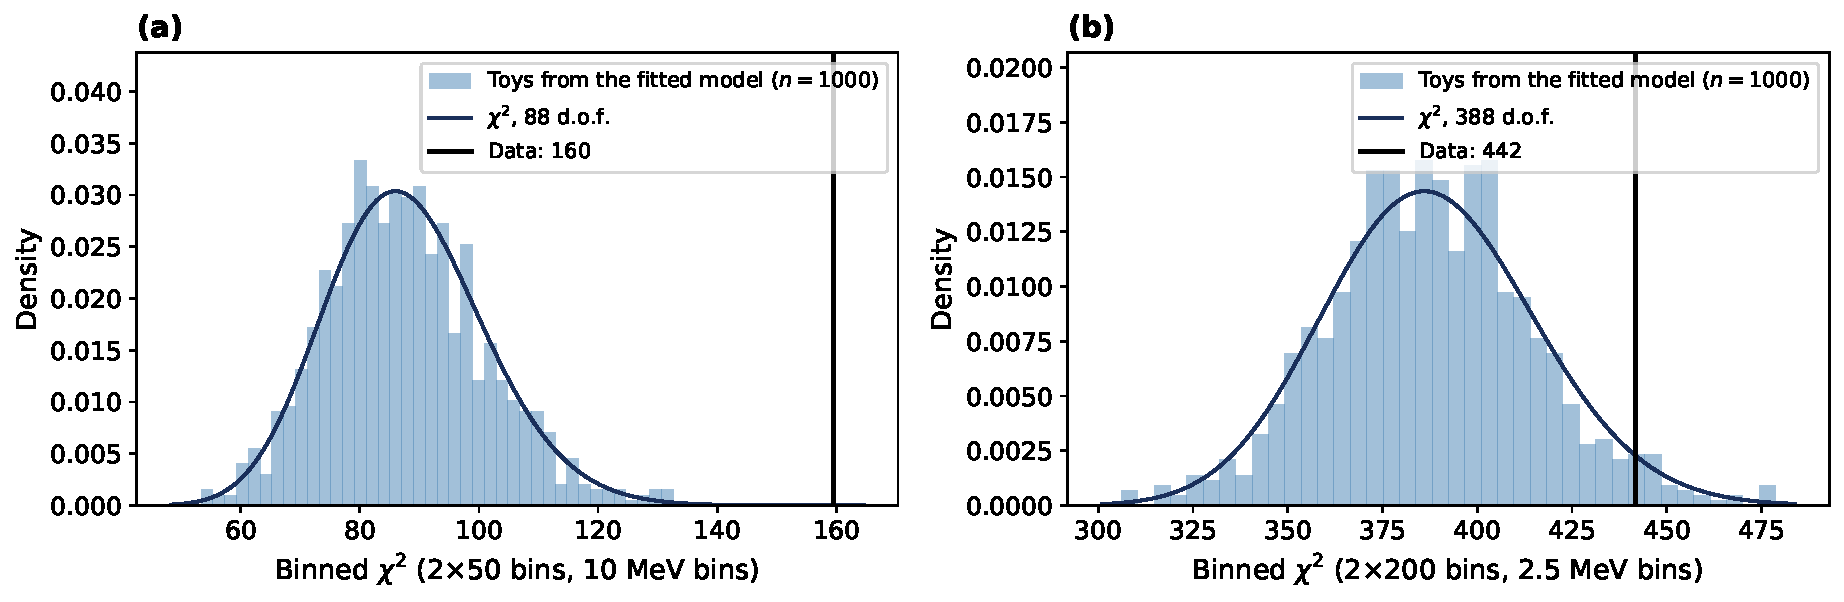
\includegraphics[width=0.95\textwidth]{figures/validation_gof_toys.pdf}
\caption{Binned $\chi^2$ of $1000$ toy-MC experiments from the fitted model, $\chi^2$ distribution with the corresponding degrees of freedom, and value of the data: (a) $2\times50$ bins of $10\,\MeV$, (b) $2\times200$ bins of $2.5\,\MeV$.}
\label{fig:validation_gof}
\end{figure*}

\FloatBarrier
